\section{$\Thsq$ MC algorithm for $\AAbar$, $\AbarB$, and $\AE$}\label{sect:AAbarAlg}

%\subsection{\TBSAT{} and \TBSATM}
In this section, we first propose an MC algorithm for the fragment $\AAbar$ with complexity $\Thsq$, thus lower than the one described in the previous section for $\AAbarB$.
%this is possible since we drop modality $\B$. 
In fact, we do not directly devise an MC algorithm; we proceed instead \emph{via a reduction to} a
$\Thsq$-complete problem,  \TBSATM{} (a restriction of \TBSAT, see~\cite{schnoebelen2003}), whose instances are complex 
circuits where some of the gates are endowed with $\NP$ oracles.
%
%(a restriction of) \TBSAT{}~\cite{SCHNOEBELEN2003}, which we have already mentioned in the introduction.
%


\subsection{The problem \TBSATM{}}

\begin{figure}[tp]
    %\resizebox{\linewidth}{!}{}
    \centering
    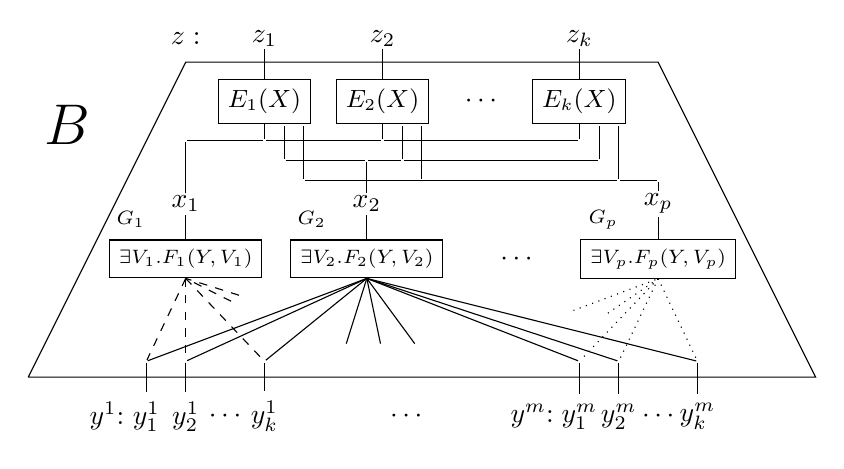
\begin{tikzpicture}
\draw (0,0) -- (10,0) -- (8,4) -- (2,4) -- (0,0);
\draw  [style={inner sep=1,outer sep=0}](0.5,3.2) node (x1) {{\huge $B$}};

\draw (2,1.5) node (f1) [draw] {\scriptsize $\exists V_1.F_1(Y,V_1)$}; \draw (1.3,2) node {{\scriptsize $G_1$}};
\draw (4.3,1.5) node (f2) [draw] {\scriptsize $\exists V_2.F_2(Y,V_2)$}; \draw (3.6,2) node {{\scriptsize $G_2$}};
\draw (6.2,1.5) node {$\cdots$};
\draw (8,1.5) node (fp) [draw] {\scriptsize $\exists V_p.F_p(Y,V_p)$}; \draw (7.3,2) node {{\scriptsize $G_p$}};

\draw  [style={inner sep=1,outer sep=0}](2,2.2) node (x1) {$x_1$};
\draw  [style={inner sep=1,outer sep=0}](4.3,2.2) node (x2) {$x_2$};
\draw  [style={inner sep=1,outer sep=0}](8,2.2) node (xp) {$x_p$};

\draw [-] (f1) -- (x1);
\draw [-] (f2) -- (x2);
\draw [-] (fp) -- (xp);

\draw (3,3.5) node [draw] (e1) {\small $E_1(X)$};
\draw (4.5,3.5) node [draw] (e2) {\small $E_2(X)$};
\draw (5.75,3.5) node {$\cdots$};
\draw (7,3.5) node [draw] (ek) {\small $E_k(X)$};

\draw  [style={inner sep=1,outer sep=0}](2,4.3) node {$\boldsymbol{z:}$};
\draw  [style={inner sep=1,outer sep=0}](3,4.3) node (z1) {$z_1$};
\draw  [style={inner sep=1,outer sep=0}](4.5,4.3) node (z2) {$z_2$};
\draw  [style={inner sep=1,outer sep=0}](7,4.3) node (zk) {$z_k$};

\draw  (e1) edge (z1);
\draw  (e2) edge (z2);
\draw  (ek) edge (zk);

\node at (1,-0.5) {$\boldsymbol{y^1}$:};
\node (v2) at (1.5,-0.5) {$y_1^1$};
\node (v4) at (2,-0.5) {$y_2^1$};
\node at (2.5,-0.5) {$\cdots$};
\node (v6) at (3,-0.5) {$y_k^1$};

\node [style={inner sep=0,outer sep=0}] (v1) at (1.5,0.2) {};
\node [style={inner sep=0,outer sep=0}] (v3) at (2,0.2) {};
\node  [style={inner sep=0,outer sep=0}](v5) at (3,0.2) {};

\node at (4.8,-0.5) {$\cdots$};

\node (v8) at (7,-0.5) {$y_1^m$};
\node (v10) at (7.5,-0.5) {$y_2^m$};
\node at (8,-0.5) {$\cdots$};
\node (v12) at (8.5,-0.5) {$y_k^m$};
\node at (6.4,-0.5) {$\boldsymbol{y^m}$:};

\node [style={inner sep=0,outer sep=0}] (v7) at (7,0.2) {};
\node [style={inner sep=0,outer sep=0}] (v9) at (7.5,0.2) {};
\node [style={inner sep=0,outer sep=0}] (v11) at (8.5,0.2) {};

\draw  (v1) edge (v2);
\draw  (v3) edge (v4);
\draw  (v5) edge (v6);
\draw  (v7) edge (v8);
\draw  (v9) edge (v10);
\draw  (v11) edge (v12);
\draw  (v1) edge (f2.south);
\draw  (v3) edge (f2.south);
\draw  (v5) edge (f2.south);
\draw  (v7) edge (f2.south);
\draw  (v9) edge (f2.south);
\draw  (v11) edge (f2.south);

\node [style={inner sep=0,outer sep=0}] (v13) at (2,3) {};
\node [style={inner sep=0,outer sep=0}] (v16) at (7,3) {};
\node [style={inner sep=0,outer sep=0}] (v19) at (3.5,2.5) {};
\node [style={inner sep=0,outer sep=0}] (v18) at (7.5,2.5) {};
\node [style={inner sep=0,outer sep=0}] (v17) at (8,2.5) {};
\node [style={inner sep=0,outer sep=0}] (v14) at (3,3) {};
\node [style={inner sep=0,outer sep=0}] (v15) at (4.5,3) {};
\draw  (x1) edge (v13);
\draw  (v13) edge (v14);
\draw  (v14) edge (v15);
\draw  (v15) edge (v16);
\draw  (v16) edge (ek);
\draw  (v15) edge (e2);
\draw  (e1) edge (v14);
\draw  (xp) edge (v17);
\draw  (v17) edge (v18);
\draw  (v18) edge (v19);
\node [style={inner sep=0,outer sep=0}] (v21) at (5,2.5) {};
\node [style={inner sep=0,outer sep=0}] (v20) at (3.5,3.2) {};
\node [style={inner sep=0,outer sep=0}] (v22) at (5,3.2) {};
\node [style={inner sep=0,outer sep=0}] (v23) at (7.5,3.2) {};
\draw  (v19) edge (v20);
\draw  (v21) edge (v22);
\draw  (v18) edge (v23);

\node [style={inner sep=0,outer sep=0}] (v25) at (3.25,2.75) {};
\node [style={inner sep=0,outer sep=0}] (v27) at (4.75,2.75) {};
\node [style={inner sep=0,outer sep=0}] (v29) at (7.25,2.75) {};
\node [style={inner sep=0,outer sep=0}] (v24) at (3.25,3.2) {};
\node [style={inner sep=0,outer sep=0}] (v28) at (4.75,3.2) {};
\node [style={inner sep=0,outer sep=0}] (v30) at (7.25,3.2) {};
\node [style={inner sep=0,outer sep=0}] (v26) at (4.3,2.75) {};
\draw  (v24) edge (v25);
\draw  (v25) edge (v26);
\draw  (v26) edge (v27);
\draw  (v27) edge (v28);
\draw  (v27) edge (v29);
\draw  (v29) edge (v30);
\draw  (v26) edge (x2);
\draw [dashed] (f1.south) edge (v1);
\draw [dashed] (f1.south) edge (v3);
\draw [dashed] (f1.south) edge (v5);
\draw [dotted] (fp.south) edge (v7);
\draw [dotted] (fp.south) edge (v9);
\draw [dotted] (fp.south) edge (v11);
\node (v32) at (2.7,0.9) {};
\node (v33) at (2.8,1) {};
\node (v31) at (7.2,0.7) {};
\node (v34) at (6.8,0.8) {};
\draw [dashed] (v32) edge (f1.south);
\draw [dashed] (v33) edge (f1.south);
\draw [dotted] (v34) edge (fp.south);
\draw [dotted] (fp.south) edge (v31);
\node (v35) at (4,0.3) {};
\node (v36) at (4.5,0.3) {};
\node (v37) at (5,0.3) {};
\draw (f2.south) edge (v35);
\draw (f2.south) edge (v36);
\draw (v37) edge (f2.south);
\end{tikzpicture}
    \caption{General form of a block.}\label{blockFig}
\end{figure}

In order to introduce \TBSAT, we need to preliminarily describe its basic component, which is the \emph{block}. A block $B$ (see Figure~\ref{blockFig}) is a circuit
%---we generically call it $B$---
whose input lines are organized in $m$ bit vectors $\boldsymbol{y^1},\ldots,\boldsymbol{y^m}$, each of which has $k$ entries, namely $\boldsymbol{y^i}=(y^i_1, \ldots ,y^i_k)$. The values $m$ and $k$ are respectively called the \emph{degree} and the \emph{width} of $B$.
The input lines are connected to $p$ internal gates $G_1,\ldots,G_p$. Each gate $G_i$
features a Boolean formula $F_i(Y,V_i)$ associated with it, where $Y=\{y^j_s\mid j=1,\dots ,m,\; s=1,\dots , k\}$ and $V_i$ is a set of private variables of $F_i$, not occurring in any other $F_j$, with $j\neq i$, that is, $V_i\cap V_j=\emptyset$ for $j\neq i$.
The gate $G_i$ queries a SAT oracle in order to decide whether the associated Boolean formula is satisfiable.
The output of $G_i$ is denoted by $x_i$, and it evaluates to $\top$ if and only if $F_i(Y,V_i)$ is satisfiable. Finally, $k$ classic circuits (without oracles) $E_1,\ldots,E_k$ compute, from $X=\{x_1, \ldots,x_p\}$, their outputs $z_1,\ldots,z_k$, which are also the final $k$ outputs of the block $B$. 
%
The size of $B$ is defined as the total number of gates, plus the lengths of all the
associated Boolean formulas.
%$F_i(Y,V_i)$'s.
%
In the following, to make clear that a gate $G_i$ (respectively, input $y_i$, block output $z_i$, gate output $x_i$) is an element of a block $B$, we write  $B(G_i)$ (respectively, $B(y_i)$, $B(z_i)$, $B(x_i)$).

Given the $k\cdot m$ input bits, determining the output value of any $z_i$ is a $\Thpar$ problem: the $p$ queries associated with the oracle gates, which determine the outputs $x_j$'s, can be performed in parallel (they are independent of each other) and then the value of the block output $z_i$ can be calculated in deterministic polynomial time.

\begin{figure}[tp]
    \centering
    \resizebox{0.8\linewidth}{!}{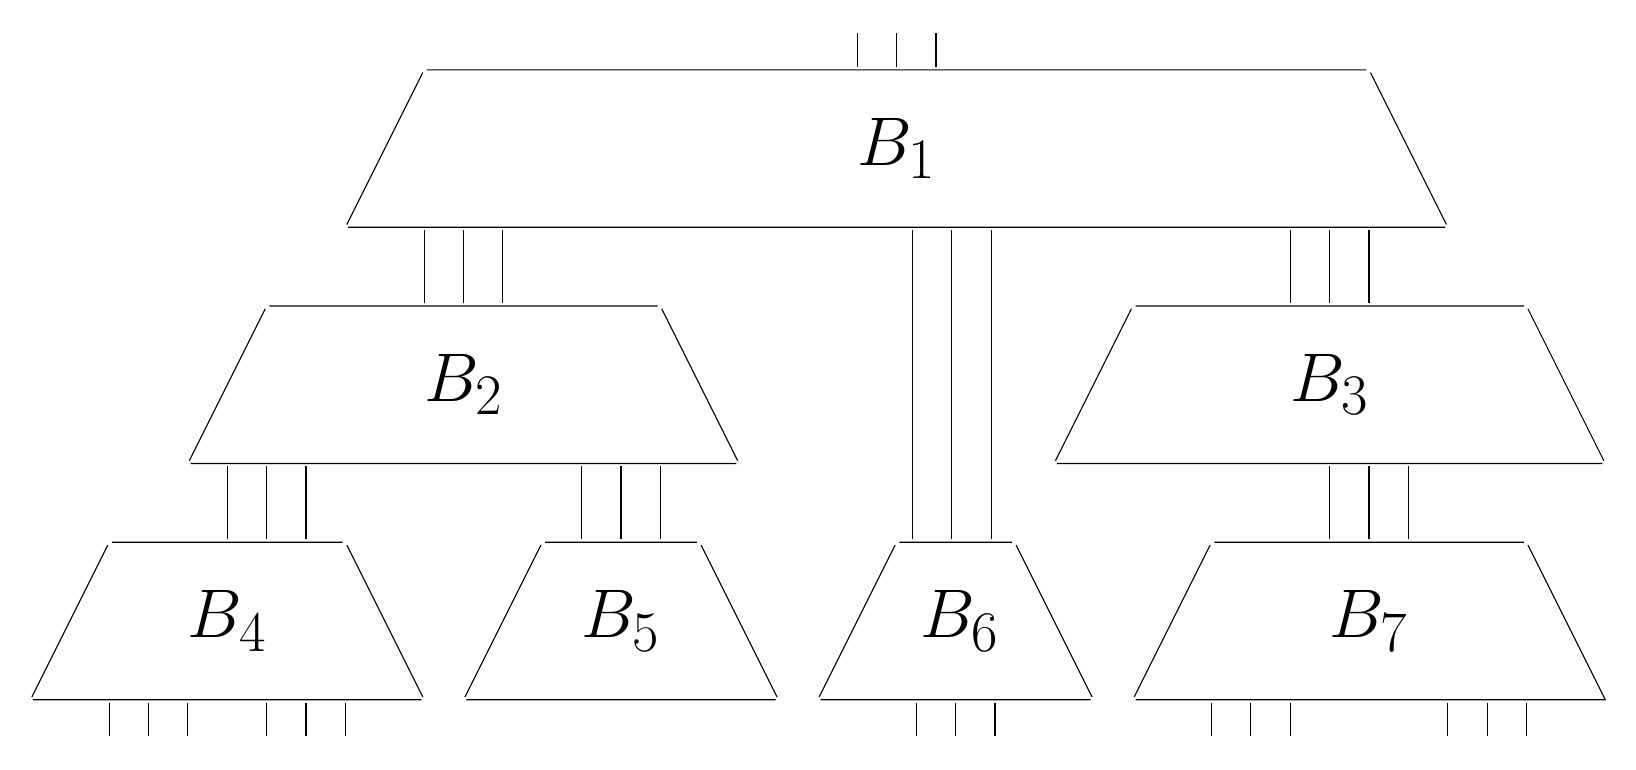
\begin{tikzpicture}

\node [style={inner sep=1,outer sep=0}] (v1) at (0,0) {};
\node [style={inner sep=1,outer sep=0}] (v2) at (14,0) {};
\node [style={inner sep=1,outer sep=0}] (v4) at (1,2) {};
\node [style={inner sep=1,outer sep=0}] (v3) at (13,2) {};
\draw (v4) -- (v1) -- (v2) -- (v3) -- (v4);

\node [style={inner sep=1,outer sep=0}] (v11) at (-2,-3) {};
\node [style={inner sep=1,outer sep=0}] (v21) at (5,-3) {};
\node [style={inner sep=1,outer sep=0}] (v41) at (-1,-1) {};
\node [style={inner sep=1,outer sep=0}] (v31) at (4,-1) {};
\draw (v41) -- (v11) -- (v21) -- (v31) -- (v41);

\node [style={inner sep=1,outer sep=0}] (v12) at (-4,-6) {};
\node [style={inner sep=1,outer sep=0}] (v22) at (1,-6) {};
\node [style={inner sep=1,outer sep=0}] (v42) at (-3,-4) {};
\node [style={inner sep=1,outer sep=0}] (v32) at (0,-4) {};
\draw (v42) -- (v12) -- (v22) -- (v32) -- (v42);

\node [style={inner sep=1,outer sep=0}] (v13) at (1.5,-6) {};
\node [style={inner sep=1,outer sep=0}] (v23) at (5.5,-6) {};
\node [style={inner sep=1,outer sep=0}] (v43) at (2.5,-4) {};
\node [style={inner sep=1,outer sep=0}] (v33) at (4.5,-4) {};
\draw (v43) -- (v13) -- (v23) -- (v33) -- (v43);

\node [style={inner sep=1,outer sep=0}] (v14) at (6,-6) {};
\node [style={inner sep=1,outer sep=0}] (v24) at (9.5,-6) {};
\node [style={inner sep=1,outer sep=0}] (v44) at (7,-4) {};
\node [style={inner sep=1,outer sep=0}] (v34) at (8.5,-4) {};
\draw (v44) -- (v14) -- (v24) -- (v34) -- (v44);

\node [style={inner sep=1,outer sep=0}] (v15) at (9,-3) {};
\node [style={inner sep=1,outer sep=0}] (v25) at (16,-3) {};
\node [style={inner sep=1,outer sep=0}] (v45) at (10,-1) {};
\node [style={inner sep=1,outer sep=0}] (v35) at (15,-1) {};
\draw (v45) -- (v15) -- (v25) -- (v35) -- (v45);

\node [style={inner sep=1,outer sep=0}] (v16) at (10,-6) {};
\node [style={inner sep=1,outer sep=0}] (v26) at (16,-6) {};
\node [style={inner sep=1,outer sep=0}] (v46) at (11,-4) {};
\node [style={inner sep=1,outer sep=0}] (v36) at (15,-4) {};
\draw (v46) -- (v16) -- (16,-6) -- (v36) -- (v46);

\node [style={inner sep=1,outer sep=0}] (v29) at (1.5,-1) {};
\node [style={inner sep=1,outer sep=0}] (v37) at (2,-1) {};
\node [style={inner sep=1,outer sep=0}] (v27) at (1,-1) {};
\node [style={inner sep=1,outer sep=0}] (v5) at (-1.5,-4) {};
\node [style={inner sep=1,outer sep=0}] (v7) at (-1,-4) {};
\node [style={inner sep=1,outer sep=0}] (v9) at (-0.5,-4) {};
\node [style={inner sep=1,outer sep=0}] (v18) at (3.5,-4) {};
\node [style={inner sep=1,outer sep=0}] (v49) at (12.5,-4) {};
\node [style={inner sep=1,outer sep=0}] (v51) at (13,-4) {};
\node [style={inner sep=1,outer sep=0}] (v53) at (13.5,-4) {};
\node [style={inner sep=1,outer sep=0}] (v59) at (12,-1) {};
\node [style={inner sep=1,outer sep=0}] (v57) at (12.5,-1) {};
\node [style={inner sep=1,outer sep=0}] (v55) at (13,-1) {};
\node [style={inner sep=1,outer sep=0}] (v28) at (1,0) {};
\node [style={inner sep=1,outer sep=0}] (v30) at (1.5,0) {};
\node [style={inner sep=1,outer sep=0}] (v38) at (2,0) {};
\node [style={inner sep=1,outer sep=0}] (v60) at (12,0) {};
\node [style={inner sep=1,outer sep=0}] (v58) at (12.5,0) {};
\node [style={inner sep=1,outer sep=0}] (v56) at (13,0) {};

\node [style={inner sep=1,outer sep=0}] (v17) at (3,-3) {};
\node [style={inner sep=1,outer sep=0}] (v19) at (3.5,-3) {};
\node [style={inner sep=1,outer sep=0}] (v20) at (4,-3) {};
\node [style={inner sep=1,outer sep=0}] (v6) at (-1.5,-3) {};
\node [style={inner sep=1,outer sep=0}] (v8) at (-1,-3) {};
\node [style={inner sep=1,outer sep=0}] (v10) at (-0.5,-3) {};
\node [style={inner sep=1,outer sep=0}] (v50) at (12.5,-3) {};
\node [style={inner sep=1,outer sep=0}] (v52) at (13,-3) {};
\node [style={inner sep=1,outer sep=0}] (v54) at (13.5,-3) {};
\node [style={inner sep=1,outer sep=0}] (v61) at (3,-4) {};
\node [style={inner sep=1,outer sep=0}] (v62) at (4,-4) {};

\draw  (v5) edge (v6);
\draw  (v7) edge (v8);
\draw  (v9) edge (v10);
\draw  (v18) edge (v19);
\draw  (v27) edge (v28);
\draw  (v29) edge (v30);
\draw  (v37) edge (v38);

\draw  (v49) edge (v50);
\draw  (v51) edge (v52);
\draw  (v53) edge (v54);
\draw  (v55) edge (v56);
\draw  (v57) edge (v58);
\draw  (v59) edge (v60);
\draw  (v17) edge (v61);
\draw  (v20) edge (v62);

\node [style={inner sep=1,outer sep=0}] (v48) at (7.7,-4) {};
\node [style={inner sep=1,outer sep=0}] (v64) at (8.2,-4) {};
\node [style={inner sep=1,outer sep=0}] (v40) at (7.2,-4) {};
\node [style={inner sep=1,outer sep=0}] (v39) at (7.2,0) {};
\node [style={inner sep=1,outer sep=0}] (v47) at (7.7,0) {};
\node [style={inner sep=1,outer sep=0}] (v63) at (8.2,0) {};
\draw  (v39) edge (v40);
\draw  (v47) edge (v48);
\draw  (v63) edge (v64);


\node [style={inner sep=1,outer sep=0}] (v65) at (-3,-6) {};
\node [style={inner sep=1,outer sep=0}] (v67) at (-2.5,-6) {};
\node [style={inner sep=1,outer sep=0}] (v69) at (-2,-6) {};
\node [style={inner sep=1,outer sep=0}] (v71) at (-1,-6) {};
\node [style={inner sep=1,outer sep=0}] (v73) at (-0.5,-6) {};
\node [style={inner sep=1,outer sep=0}] (v75) at (0,-6) {};
\node [style={inner sep=1,outer sep=0}] (v66) at (-3,-6.5) {};
\node [style={inner sep=1,outer sep=0}] (v68) at (-2.5,-6.5) {};
\node [style={inner sep=1,outer sep=0}] (v70) at (-2,-6.5) {};
\node [style={inner sep=1,outer sep=0}] (v72) at (-1,-6.5) {};
\node [style={inner sep=1,outer sep=0}] (v74) at (-0.5,-6.5) {};
\node [style={inner sep=1,outer sep=0}] (v76) at (0,-6.5) {};
\node [style={inner sep=1,outer sep=0}] (v77) at (7.25,-6) {};
\node [style={inner sep=1,outer sep=0}] (v79) at (7.75,-6) {};
\node [style={inner sep=1,outer sep=0}] (v81) at (8.25,-6) {};
\node [style={inner sep=1,outer sep=0}] (v83) at (11,-6) {};
\node [style={inner sep=1,outer sep=0}] (v85) at (11.5,-6) {};
\node [style={inner sep=1,outer sep=0}] (v87) at (12,-6) {};
\node [style={inner sep=1,outer sep=0}] (v89) at (14,-6) {};
\node [style={inner sep=1,outer sep=0}] (v91) at (14.5,-6) {};
\node [style={inner sep=1,outer sep=0}] (v93) at (15,-6) {};
\node [style={inner sep=1,outer sep=0}] (v84) at (11,-6.5) {};
\node [style={inner sep=1,outer sep=0}] (v86) at (11.5,-6.5) {};
\node [style={inner sep=1,outer sep=0}] (v88) at (12,-6.5) {};
\node [style={inner sep=1,outer sep=0}] (v90) at (14,-6.5) {};
\node [style={inner sep=1,outer sep=0}] (v92) at (14.5,-6.5) {};
\node [style={inner sep=1,outer sep=0}] (v94) at (15,-6.5) {};
\node [style={inner sep=1,outer sep=0}] (v82) at (8.25,-6.5) {};
\node [style={inner sep=1,outer sep=0}] (v80) at (7.75,-6.5) {};
\node [style={inner sep=1,outer sep=0}] (v78) at (7.25,-6.5) {};
\draw  (v65) edge (v66);
\draw  (v67) edge (v68);
\draw  (v69) edge (v70);
\draw  (v71) edge (v72);
\draw  (v73) edge (v74);
\draw  (v75) edge (v76);
\draw  (v77) edge (v78);
\draw  (v79) edge (v80);
\draw  (v81) edge (v82);
\draw  (v83) edge (v84);
\draw  (v85) edge (v86);
\draw  (v87) edge (v88);
\draw  (v89) edge (v90);
\draw  (v91) edge (v92);
\draw  (v93) edge (v94);


\node [style={inner sep=1,outer sep=0}] (v97) at (7,2) {};
\node [style={inner sep=1,outer sep=0}] (v95) at (6.5,2) {};
\node [style={inner sep=1,outer sep=0}] (v99) at (7.5,2) {};
\node [style={inner sep=1,outer sep=0}] (v96) at (6.5,2.5) {};
\node [style={inner sep=1,outer sep=0}] (v98) at (7,2.5) {};
\node [style={inner sep=1,outer sep=0}] (v100) at (7.5,2.5) {};
\draw [style={inner sep=1,outer sep=0}]  (v95) edge (v96);
\draw [style={inner sep=1,outer sep=0}]  (v97) edge (v98);
\draw [style={inner sep=1,outer sep=0}]  (v99) edge (v100);


\node at (7,1) {\Huge $B_1$};
\node at (1.5,-2) {\Huge $B_2$};
\node at (12.5,-2) {\Huge $B_3$};
\node at (-1.5,-5) {\Huge $B_4$};
\node at (3.5,-5) {\Huge $B_5$};
\node at (7.8,-5) {\Huge $B_6$};
\node at (13,-5) {\Huge $B_7$};
\end{tikzpicture}
}
        
    %\vspace*{0.45cm}
    \caption{A tree of blocks ($B_5$ has degree $m=0$).}\label{tob}
\end{figure}%

Blocks of \emph{the same width} can be combined together to form a tree-structured complex circuit, called a \emph{tree of blocks}. See Figure~\ref{tob} for an example.
%
Every block in the tree-structure has a level: blocks which are leaves of the tree are at level 1;
%if the inputs of $B_i$ do not depend on the outputs of any other $B_j$, then its level is 1 (such a $B_i$ is a leaf of the tree); 
a block $B_i$ whose inputs depend on (at least) a block $B_j$ at level $d-1$ and possibly on other blocks at levels less than $d$, is at level $d$. In Figure~\ref{tob}, 
$B_4$, $B_5$, $B_6$, $B_7$ are at level 1,
$B_2$ and $B_3$ at level 2, 
and $B_1$ at level 3. 
If the root of the tree-structure $T$ is at level $d$, the $k$ outputs of $T$ can be determined by $d$ rounds of parallel queries: all the queries relative to blocks placed at the same level $d'$ can be answered in parallel once all those at level $d'-1$ have been answered. 

\TBSAT{} is the problem of deciding whether a specific output $z_i$ of (the root of) a tree-structure of blocks $T$ is $\top$ or $\bot$, given the values for the inputs (of the leaf blocks) of $T$. As proved in~\cite{schnoebelen2003}, the problem \TBSAT{} is $\PTIME^{\NP}$-complete.

The problem \TBSATM{} is a constrained version of \TBSAT{}: any Boolean formula (SAT query) associated with a block $B$ of the tree-structure must have the following form: \[\exists\ell_1,\ldots ,\ell_m\in\{1,\ldots ,k\}\,\exists V'_i.F_i(y^1_{\ell_1},\ldots ,y^m_{\ell_m},\ell_1,\ldots ,\ell_m,V'_i),\] where $m$ and $k$ are respectively the degree and the width of $B$. This amounts to say that $F_i$ can use \emph{only one bit from each input vector} of $B$ (no matter which), hence ``$1\times M$''. 
The existential quantification over the indexes $\ell_1,\ldots ,\ell_m$ is an abuse of notation borrowed from~\cite{schnoebelen2003}: %however 
$\exists\ell_j\in\{1,\ldots ,k\}$ is just a shorthand for $k$ bits (belonging to the set of private variables) ``$\ell_j=1$'', \dots , ``$\ell_j=k$'', among which exactly one is $\top$. In the  formula above, $V'_i$ is $V_i$ deprived of such bits.%\footnote{un po faticosa la spiegazione bisognerebbe lavorarci}

In~\cite{schnoebelen2003}, it is proved that \TBSATM{} is a $\Thsq$-complete problem. In particular, the proof of membership to $\Thsq$ exploits the \emph{squeeze} technique of~\cite{gottlob1995} applied to TREE(SAT) instances.  The particular form ``$1\times M$'' of the queries allows us to \lq\lq reshape\rq\rq{} the tree-structure of blocks, in such a way that the height becomes logarithmic in the number of blocks. Therefore, only $O(\log n)$ rounds of parallel queries are needed, allowing us to prove membership of the problem to $\Thparlogn=\Thsq$.
%basically, whenever a block $B$ at level $d$ has only a child $B'$ at level $d-1$---but may have other children at levels $\leq d-2$---$B$ and $B'$ can be merged by exploiting the particular ``$1\times M$'' form of queries. By repeating these fusions, the height of the tree can be made logarithmic, thus only $O(\log n)$ rounds of parallel queries are needed: membership to $\Thparlogn=\Thsq$ follows.


\subsection{Reduction of MC for $\AAbar$ to \TBSATM }
Let us show now how to reduce the MC problem for $\AAbar$ formulas to \TBSATM . 
%showing how to build a suitable tree of blocks that allows us to decide the former problem.
As in the previous section, w.l.o.g., we assume that  only \emph{existential} modalities occur 
in the $\AAbar$ formula $\psi$ to be checked over a Kripke structure $\Ku=(\Prop,\States,\Edges,\Lab,s_1)$, 
with $\States=\{s_1,\ldots , s_{|\States|}\}$.\footnote{Here, for technical reasons, we assume an arbitrary order of the states of the Kripke structure, $s_1,\ldots , s_{|\States|}$, where $s_1$ is the initial state.}
We consider its negation $\neg\psi$ and build from it a tree-structure of blocks $T_{\Ku,\neg\psi}$.
%
Each block of $T_{\Ku,\neg\psi}$ has a type, \forw{} or \back, and it is associated with a subformula of $\neg\psi$. The root block, $B_{root}$, is always of type \forw\ and it is associated with $\neg\psi$. Each block $B$ has an output line $z_i$ for each state $s_i\in \States$, thus the \emph{width} of all blocks is $k=|\States|$.
%Every block of $T_{\Ku,\neg\psi}$ is associated with \emph{modal sub-formulas}
%of $\neg\psi$. 

Starting from $B_{root}$,  $T_{\Ku,\neg\psi}$ is built by recursive applications of the following \emph{basic step}, 
which are guided
%(just like in Algorithm~\ref{MC})
by the $\AAbar$-modal subformulas (recall Definition~\ref{def:modsubf}):
%
if some (generic) block $B$ is associated with a formula $\varphi$, then
\begin{itemize}
	\item for every $\phi\in\mods(\varphi)$, where $\phi = \hsA \xi$, we create a \forw{} child $B'$ of $B$ associated with $\xi$, and
	\item for every $\phi'\in\mods(\varphi)$, where $\phi' = \hsAt \xi'$, we create a \back{} child $B''$ of $B$ associated with $\xi'$.
\end{itemize}
Then, the basic step is recursively applied to all the generated children of $B$, terminating when $\mods(\varphi)=\emptyset$.
Note that a block $B$ associated with a formula $\varphi$ has \emph{degree} $m=|\mods(\varphi)|$.

In such a way, we determine the 
%\lq\lq external\rq\rq{} 
tree-structure of blocks $T_{\Ku,\neg\psi}$. We now describe the internal structure of blocks. 

As a preliminary step, we suitably transform $\AAbar$ formulas $\varphi$ into Boolean ones by replacing all the occurrences of proposition letters and modal subformulas in $\varphi$ by Boolean variables, as described by the next definition.

\begin{definition}\label{psioverl}
Let $\Ku=(\Prop,\States,\Edges,\Lab,s_1)$ be a finite Kripke structure and let $\chi$ be
an $\AAbar$ formula. We define $\overline{\chi}(V_\Prop, V_{modSubf})$---where $V_\Prop=\{v_p\mid p\in\Prop\}$ and $V_{modSubf}=\{v_{\chi'}\mid\chi'\in\mods(\chi)\}$ are sets of Boolean variables---as the \emph{Boolean} formula obtained from $\chi$ by replacing
\begin{itemize}
	\item each (occurrence of a) $\AAbar$-modal subformula $\chi'\in \mods(\chi)$ by the variable $v_{\chi'}$,
	\item and \emph{subsequently} each (occurrence of a) proposition letter $p\in\Prop$ by the variable $v_p$.
\end{itemize}
\end{definition}

Given a trace $\rho\in\Trk_\Ku$ and an $\AAbar$ formula $\chi$,
it is easy to prove (by induction on the complexity of $\overline{\chi}(V_\Prop,V_{modSubf})$) that
if $\omega$ is an interpretation (truth assignment) of the variables of $V_\Prop\cup V_{modSubf}$ such that $\omega(v_p)=\top\iff \Ku,\rho\models p$, for all $p\in\Prop$, and $\omega(v_{\chi'})=\top\iff \Ku,\rho\models \chi'$, for all $\chi'\in\mods(\chi)$, then it holds that $\Ku,\rho\models \chi\iff\omega(\overline{\chi}(V_\Prop,V_{modSubf}))=\top$.
%\footnote{la valutazione omega sulla formula e' un abuso di notazione lo vogliamo tenere?)}

We are now ready to describe the internal structure of a block $B$ for a formula $\varphi$ in $T_{\Ku,\neg\psi}$. Let us assume that $B$ has type \forw{} and let us refer  to the block depicted in Figure~\ref{blockFig} for the description. The block features a gate $G_i$, with $1 \leq i \leq |\States|$, for each state of $\Ku$. Each output line $z_i$ of $B$ is directly linked to the output $x_i$ of the oracle gate $G_i$, avoiding the use of circuits $E_1,\ldots,E_k$.
%$T_{\Ku,\neg\psi}$. 

Now, let $F_i(Y,V)$ be the Boolean formula for the gate $G_i$, with $1\leq i\leq |\States|$ (for the sake of simplicity, we write $V$ instead of $V_i$). The basic idea is that $F_i(Y,V)$ is satisfiable if and only if there is a trace having length at most $|\States|^2+2$, starting from the $i$-th state of $\States$, which satisfies $\overline{\varphi}(V_{\Prop},V_{modSubf})$, where $\varphi$
is the formula associated with the block $B$. To check the existence of such a witness trace,  we need a set of private variables $V_{trace}=\{v_1^1, \ldots, v_{|\States|}^1, v_1^2, \ldots, v_{|\States|}^2, \ldots, v_1^{|\States|^2+2}, \ldots, v_{|\States|}^{|\States|^2+2}\}$. In particular, 
the subset of variables $v_1^j, \ldots, v_{|\States|}^j$, with $1 \leq j \leq |\States|^2+2$, 
is used to \lq\lq encode\rq\rq{} the state in the $j$-th position of the trace. The encoding requires that exactly one variable $v_k^j$ of the subset is assigned to $\top$, for $1 \leq k \leq |\States|$, meaning that the $k$-th state of $\Ku$ occurs in the $j$-th position of the sequence.
%
Moreover, we use a set of private variables $V_{last}=\{v_1, v_2, \ldots, v_{|\States| }\}$ which are used to encode the last state of the witness trace (note that the length of the witness trace can be actually less than the bound  $|\States|^2+2$).

In detail, the Boolean formula $trace(V_{trace},V_{last},V_{\Prop})$, which ensures
that a truth assignment of the private variables
$V_{trace}$ properly encodes a trace $\rho$ of $\Ku$ of length $\ell$, for $1 \leq \ell \leq |\States|^2+2$, is as follows.

\begin{multline*}
trace(V_{trace},V_{last},V_{\Prop})=
\bigvee_{\ell=1}^{|\States|^2+2}
\Big[\bigwedge_{t=1}^{\ell} one_t(v_1^t, v_2^t, \ldots, v_{|\States|}^t) \wedge \\
\bigwedge_{t=1}^{\ell-1} edge_t(v_1^t, \ldots ,v_{|\States|}^t,v_1^{t+1}, \ldots ,v_{|\States|}^{t+1}) \wedge
\underbrace{\bigwedge_{t=1}^{|\States|} (v^\ell_t \leftrightarrow v_t)}_{(1)} \wedge\\
\underbrace{\bigwedge_{p\in\Prop}\!\! \Big(\big(v_p \!\rightarrow\! \bigwedge_{t=1}^\ell \bigwedge_{j=1}^{|\States|}(v_j^t\!\rightarrow\! VAL(s_j,p))\big) \!\wedge\! \big(\neg v_p \!\rightarrow\! \bigvee_{t=1}^\ell \bigwedge_{j=1}^{|\States|}(v_j^t\!\rightarrow\! \neg VAL(s_j,p))\big)\Big)}_{(2)}
\Big].
\end{multline*}

For any $1 \leq t \leq \ell$, being $\ell$ the length of 
the witness trace, the Boolean formula $one_t(v_1^t, v_2^t, \ldots, v_{|\States|}^t)$ \lq\lq checks\rq\rq{} that the variables  $v_1^t, v_2^t, \ldots, v_{|\States|}^t$ encode (exactly) one state for the $t$-th element of the trace:
\[one_t(v_1^t, v_2^t, \ldots, v_{|\States|}^t)=\Big(\bigvee_{j=1}^{|\States|}v_j^t\Big) \wedge\Big(\bigwedge_{j=1}^{|\States|}\bigwedge_{k=j+1}^{|\States|}\neg(v_j^t \wedge v_k^t)\Big).\]
Then, for any $1 \leq t \leq \ell -1$, the formula $edge_t(v_1^t, \ldots ,v_{|\States|}^t,v_1^{t+1}, \ldots ,v_{|\States|}^{t+1})$ checks that
if $s_k$ and $s_j$ are states which occur consecutively in the encoded trace ($v_k^t$ and $v_j^{t+1}$ are set to $\top$), then 
$(s_k,s_j)\in\Edges$:
\[edge_t(v_1^t, \ldots ,v_{|\States|}^t,v_1^{t+1}, \ldots ,v_{|\States|}^{t+1})=\smashoperator{\bigvee_{(s_k,s_j)\in\Edges}} (v_k^t \wedge v_j^{t+1}).\] 
Then, conjunct (1) ensures that the private variables in $V_{last}$ encode the last state of the witness trace, that is, the $\ell$-th state.
%
%and $\{v^\ell_1,\ldots,v^\ell_{|\States|}\}$ to pairwise have the same truth value (note that $v^\ell_1,\ldots,v^\ell_{|\States|}$ \lq\lq encode\rq\rq{} the last state of a trace whose length is $\ell$).
Finally, conjunct (2) enforces the homogeneity assumption, ensuring that a variable $v_p \in V_{\Prop}$ evaluates to $\top$ if and only if $p$ holds over all the states of the witness trace ($VAL(s_j,p)$ is just a shorthand for $\top$ if $p\in\Lab(s_j)$, and $\bot$ otherwise).

%$\rho$ \lq\lq selected\rq\rq{} by the conjuncts $one_t$ and $edge_t$, for $t\geq 1$.

Now, taking the set of private variables $V= V_{last} \cup V_{trace} \cup V_{\Prop} \cup V_{modSubf}$, the Boolean formula $F_i(Y,V)$ for the gate $G_i$ is formally defined as:
\begin{multline*}
F_i(Y,V)=%\exists V\Big(
v_i^1 \wedge 
\overline{\varphi}(V_{\Prop},V_{modSubf}) \wedge
trace(V_{trace},V_{last},V_{\Prop}) \wedge 
\\
\smashoperator{\bigwedge_{\hsA\xi\in\mods(\varphi)}}\big(v_{\hsA\xi}\leftrightarrow \bigvee_{j=1}^{|\States|} (v_j \wedge y_j^\xi)\big) \quad \wedge \quad \smashoperator{\bigwedge_{\hsAt\xi'\in\mods(\varphi)}}\big(v_{\hsAt\xi'}\leftrightarrow \bigvee_{j=1}^{|\States|} (v_j^1 \wedge y_j^{\xi'})\big)
%\Big).
\end{multline*}
%where  $V= V_{last} \cup V_{trace} \cup V_{\Prop} \cup V_{modSubf}$ is the set of (private) variables, with
%\begin{itemize}
%    \item $V_{last}=\{v_1, v_2, \ldots, v_{|\States|}\}$,
  %  \item $V_{trace}=\{v_1^1, \ldots, v_{|\States|}^1, v_1^2, \ldots, v_{|\States|}^2, \ldots, v_1^{|\States|^2+2}, \ldots, v_{|\States|}^{|\States|^2+2}\}$, and 
  %  \item $V_\Prop$, $V_{modSubf}$ and $\overline{\varphi}(V_{\Prop},V_{modSubf})$ are as in Definition \ref{psioverl}.
%\end{itemize}
 
The first conjunct of $F_i(Y,V)$ requires that the witness trace starts with the $i$-th state of $\Ku$. The fourth one requires that each private variable $v_{\hsA\xi}$, for $\hsA\xi \in\mods(\varphi)$ has exactly the same truth assignment as the $j$-th output, $y_j^\xi$, of the block for $\xi$
(which is a child of $B$)---provided that the final state of the trace is the $j$-th state of $\Ku$.
Since exactly one among the variables of $V_{last}=\{v_1,\ldots , v_{|\States|}\}$ is set to $\top$, it is guaranteed that at most one bit for every child-block is considered by $B$, thus fulfilling the restriction of \TBSATM. The last conjunct of $F_i(Y,V)$ forces the symmetric constraint for modal subformulas of the form $\hsAt\xi'$.

The formula $F_i(Y,V)$ for a gate $G_i$ in a \back{} block is very similar: we just need to replace the first conjunct $v_i^1$ by $v_i$.

The following proposition states the correctness of the encoding for traces.

\begin{proposition}\label{remk}
Given a trace $\rho\in\Trk_\Ku$, with $|\rho|\leq |\States|^2+2$, 
there exists a truth assignment $\omega$ to the variables in $V$ which satisfies the formula $trace(V_{trace},V_{last},V_{\Prop})$, and 
\begin{itemize}
\item for any $1 \leq t \leq |\rho|$ and $1 \leq j \leq |\States|$, $\rho(t)\!=\!s_j\!\iff\!\omega(v_j^t)\!=\!\top$ and $\omega(v_j^{|\rho|})=\omega(v_j)$;
\item for any $p\in\Prop$, $\omega(v_p)=\top\iff\Ku,\rho\models p.$
\end{itemize}
%
Conversely,
if a truth assignment $\omega$ to the variables in $V$ satisfies the $r$-th disjunct of $trace(V_{trace},V_{last},V_{\Prop})$,
then there exists a trace $\rho\in\Trk_\Ku$, with $|\rho|=r$, such that
\begin{itemize}
\item for any $1 \leq t \leq |\rho|$ and $1 \leq j \leq |\States|$, $\rho(t)=s_j\iff\omega(v_j^t)=\top$;
\item for any $p\in\Prop$, $\Ku,\rho\models p\iff\omega(v_p)=\top.$
\end{itemize}
\end{proposition}

%Finally, let us go back to $F_i(Y,V)$, and focus on the last two conjuncts. The first of them enforces the following constraint: for each $\hsA\xi\in\mods(\varphi)$, the truth values of $v_{\hsA\xi}$ and $\bigvee_{j=1}^{|\States|} (v_j \wedge y_j^{\xi})$ have to coincide, that is, $v_{\hsA\xi}$ must be assigned $\top$ if and only if, for some $j$, $v_j \wedge y_j^{\xi}$ is $\top$. Since exactly one among the variables of $V_{last}=\{v_1,\ldots , v_{|\States|}\}$ is set to $\top$, say $v_j$ (hence, $\lst(\rho)=s_j$), then $v_{\hsA\xi}$ must coincide with $y_j^{\xi}$, i.e., the $j$-th output of the child of $B$ for $\xi$. This also guarantees that at most one bit for every child-block is considered by $B$ (thus we are respecting the constraint of \TBSATM). The last conjunct of $F_i(Y,V)$ forces the symmetric constraint for modal subformulas of the form $\hsAt\xi'$.

The following theorem states the correctness of the construction of $T_{\Ku,\neg\psi}$ (the proof is given in Appendix~\ref{proof:th:cx}).

\begin{theorem}\label{th:cx} 
Let $\psi$  be an $\AAbar$ formula and  $\Ku=(\Prop,\States,\Edges,\Lab,s_1)$ be a finite Kripke structure.
For every block $B$ of $T_{\Ku,\neg\psi}$,
if $B$ is associated with an $\AAbar$ formula $\varphi$, then
\begin{itemize}
	\item if $B$ is a \forw{} block, for all $i\in\{1,\ldots,|\States|\}$, $B(z_i)=\top$ if and only if there exists a trace $\rho\in\Trk_\Ku$ such that $\fst(\rho)=s_i$ and $\Ku,\rho\models\varphi$;
	\item if $B$ is a \back{} block, for all $i\in\{1,\ldots,|\States|\}$, $B(z_i)=\top$ if and only if there exists a trace $\rho\in\Trk_\Ku$ such that $\lst(\rho)=s_i$ and $\Ku,\rho\models\varphi$.
\end{itemize}
\end{theorem}


The two next corollaries immediately follow.

\begin{corollary}\label{CorAAbar}
Let $\psi$ be an $\AAbar$ formula, $\Ku$
%=(\Prop,\States, \Edges,$ $\Lab,s_1)$
be a finite Kripke structure,
and $B_{root}$ be the root block of $T_{\Ku,\neg\psi}$. Then, it holds that
$B_{root}(z_1)=\bot$ if and only if $\Ku\models\psi$.
%\[B_{root}(z_1)=\bot\iff\Ku\models\psi.\]
\end{corollary}

\begin{corollary}\label{th:AAbaralgo}
The MC problem for $\AAbar$ formulas over finite Kripke structures is in $\Thsq$.
\end{corollary}
\begin{proof}
The result follows from Corollary~\ref{CorAAbar} and the fact that the instance of \TBSATM{} generated from an $\AAbar$ formula $\psi$ and 
a Kripke structure $\Ku$ is polynomial in $|\psi|$ and $|\Ku|$.
\end{proof}

\subsection{Reduction of MC for $\AbarB$ (resp., $\AE$) to \TBSATM }

We conclude the section by showing that it is possible to adapt the above-described reduction to the fragment $\AbarB$ and the symmetric fragment $\AE$.
%(without any complexity change).
Let us focus on $\AbarB$ (the case for $\AE$ can be dealt with in an analogous way).

Having in mind that $\AbarB$ is a fragment of $\AAbarB$, by removing the case for modality $\hsA$ in Algorithm~\ref{Oracle}, we get a procedure for which Lemma~\ref{lemmaOracle} still holds. 
Since Algorithm~\ref{Oracle} is in $\NP$, there must exist a reduction to SAT, that is, given an instance $(\Ku,\psi,s,\textsc{direction},V_{\Abar})$ for \texttt{Oracle}, there exists a Boolean formula $\Psi_{(\Ku,\psi,s,\textsc{direction},V_{\Abar})}$, which depends on $(\Ku,\psi,s,$ $\textsc{direction}, V_{\Abar})$, that is satisfiable if and only if \texttt{Oracle}$(\Ku,\psi,s,\allowbreak \textsc{direction}, V_{\Abar})$ admits a successful computation on the given input. 
By Lemma~\ref{lemmaOracle}, this is the case if and only if:  
\begin{itemize}
	\item there exists $\rho\in\Trk_{\Ku}$ such that $\fst(\rho)=s$ and $\Ku,\rho\models \psi$, in the case \textsc{direction} is \textsc{forward};
	\item there exists $\rho\in\Trk_{\Ku}$ such that $\lst(\rho)=s$ and $\Ku,\rho\models \psi$, in the case \textsc{direction} is \textsc{backward},
\end{itemize}
provided that 
for each $\hsAt \phi\in\mods(\psi)$ and $s'\in \States$, $V_{\Abar}(\phi,s')=\top$ if and only if there exists $\rho'\in\Trk_{\Ku}$ such that $\lst(\rho')=s'$ and $\Ku,\rho'\models \phi$.

The idea is that such a formula $\Psi_{(\Ku,\psi,s,\textsc{direction},V_{\Abar})}$ can be used as a SAT query for an oracle gate $G_i$ in a generic block associated with the formula $\psi$. The role of the global Boolean vector $V_{\Abar}$ is instead played by the local communication among blocks in the tree-structure; 
$\Psi_{(\Ku,\psi,s,\textsc{direction},V_{\Abar})}$ %which encodes a call to the  Algorithm~\ref{Oracle}, 
basically has the same structure as the Boolean formula $F_i(Y,V)$, with some minor differences outlined below.

First of all, we observe that Algorithm~\ref{Oracle} works with traces whose length is bounded by $|\States|\cdot (2|\psi|+1)^2$ (instead of ${| \States |}^2+ 2$ as in $F_i(Y,V)$). A trace is then encoded exactly as in $F_i(Y,V)$ by using a set of private variables
$V_{trace}=\{v_j^t \mid j=1,\ldots ,|\States|$, $t=1,\ldots , |\States|\cdot (2|\psi|+1)^2 \}$;
%
$\Psi_{(\Ku,\psi,s,\textsc{direction},V_{\Abar})}$ has also to encode the Boolean table $T$ of \texttt{Oracle} with entries $T[\varphi,i]$, where $\varphi$ is a subformula of $\psi$, and $1 \leq i \leq |\States|\cdot (2|\psi|+1)^2$ is the length of a prefix of the considered trace. Therefore,
there is a variable $x_{\varphi,i}$ in  $\Psi_{(\Ku,\psi,s,\textsc{direction},V_{\Abar})}$ for each entry $T[\varphi,i]$, with the intuitive meaning that $x_{\varphi,i}$ is assigned $\top$ if and only if $T[\varphi,i]=\top$. Actually, in this encoding we do not need any entry for a modal subformula $\hsAt \xi$, whose truth value is conveyed by $y_j^\xi$, namely, the $j$-th input connected to the child block for the subformula $\xi$ (assuming that the starting state of the trace is the $j$-th state of $\Ku$).

It is worth noting that this construction is possible since all the prefixes of the trace $\rho$ encoded by the assignment to $V_{trace}$, 
%$\tilde{\rho}\in\Pref(\rho)$ 
and $\rho$ itself, share the same starting point, and thus agree on the truth value of any $\Abar$-modal subformula. The most relevant consequence of this property is that  the constraint of \TBSATM{} on the form of SAT queries is respected.



%\begin{itemize}
%    \item For any  $j=1,\ldots ,|\States|$ and $t=1,\ldots , |\States|\cdot (2|\psi|+1)^2$, there exists a variable $v_j^t$ in  $\Psi_{(\Ku,\psi,v,\textsc{direction},V_{\Abar})}$ with the same meaning as before; however note the different bound $|\States|\cdot (2|\psi|+1)^2$, since now we apply Proposition \ref{prop:TH10};
 %   \item the subformula $trace$ still gives the encoding of a trace $\rho$, but now its length is at most $|\States|\cdot (2|\psi|+1)^2$; additionally, $trace$ determines which are the proposition letters that hold on each prefix $\tilde{\rho}\in\Pref(\rho)$, as we also have to deal with $\hsB$-subformulas.
 %   \item For each entry $T[\varphi,i]$ of $T$ (the Boolean table of \texttt{Oracle}) there is a variable $x_{\varphi,i}$ in  $\Psi_{(\Ku,\psi,v,\textsc{direction},V_{\Abar})}$ such that $x_{\varphi,i}$ is assigned $\top$ if and only if $T[\varphi,i]=\top$ (recall that $\varphi$ denotes a subformula of $\psi$, and $i$ the length of a prefix of $\rho$). An exception to this is given by the $\Abar$-modal subformulas $\xi$, whose entries $T[\xi,i]$ are all \lq\lq replaced\rq\rq{} (i.e., for all $i$) by $y_j^\xi$, where $\fst(\rho)=w_j$; %, the input of $B$ linked to the $j$-th output of the child $B'$ associated with the formula $\xi$;
%    we do this since all prefixes $\tilde{\rho}\in\Pref(\rho)$ and $\rho$ itself, sharing the same left endpoint, agree on the truth value of any $\Abar$-modal subformula.    
%\end{itemize}
%A consequence of the last point is that, again, we are respecting the constraint of \TBSATM{} on the form of SAT queries.

As for the construction of $T_{\mathpzc{K},\neg\psi}$, it is exactly as before where, in particular, the root block $B_{root}$ has type \forw, and all the other blocks have type \back. 

The following result can be stated. 
%
\begin{theorem}\label{th:AbarBalgo}
The MC problem for $\AbarB$ (resp., $\AE$) formulas over finite Kripke structures is in $\Thsq$.
\end{theorem}

The construction we have sketched cannot be adapted to the fragment $\AB$. This is due to the fact that the \emph{right} endpoints of the prefixes of a trace differ in general, and thus they do not necessarily agree on the truth value of $\A$-modal subformulas, hence the restriction of \TBSATM{} on the form of SAT queries cannot be respected.
In the next section, we will prove that MC for $\AB$ formulas is indeed \emph{inherently} more difficult than MC for $\AbarB$.
%
%thus requiring a \lq\lq more powerful\rq\rq{} \TBSAT{} tree (instead of a \TBSATM{} one) for the reduction. In the next section we will prove that model checking for $\AB$ formulas is indeed \emph{inherently} more difficult than model checking for $\AbarB$.